%describe the tasks to be completed that will satisfy the given objective
\section{Activity}
This section will give you information on the actual work necessary to complete the lab. The Background Information section will provide suplementary information and the Implementation section will provide guidelines for completing the lab.
\subsection{Background Information}
For this lab, you will be using the \verb=MediaPlayer= and \verb=MediaRecorder= classes. These classes contain methods that utilize the Android's microphone and speakers to play and record media. Before you begin the activity, visit \textit{http://developer.android.com/reference/android/media/MediaPlayer.html} and \textit{http://developer.android.com/reference/android/media/MediaRecorder.html}. Familiarize yourself with both of these classes and their methods.

The alarm system app should be able to listen for sound and, if detected, sound an alarm. There will be three different choices for the alarm sound. The following picture shows the GUI (graphical user interface) of the app:
\begin{center}

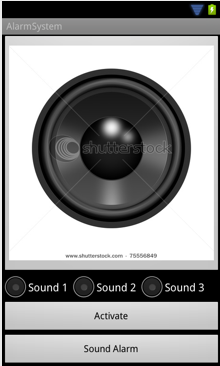
\includegraphics[scale=0.4]{screenshot.png} 

\end{center}

Both the speaker picture and the sound alarm buttons will be programmed to sound the alarm when clicked. The activate button will be programmed to begin listening for sound when clicked.


\subsection{Implementation}
This section will guide you through the implementation of the solution.
\subsubsection{Research}
Research the \verb=MediaPlayer= and \verb=MediaRecorder= classes and methods. List which methods you believe will be crucial in programming the alarm system.

\subsubsection{Explore}
Open the \verb=AlarmSystemActivity.java= file. Explore the file. Read the comments. Note the parts of the code that you will be required to fill in. They will be labeled.

\subsubsection{Import}
In order to use the classes and methods from APIs, you have to import the required libraries. Import the \verb=MediaPlayer= and \verb=MediaRecorder= libraries.

\subsubsection{Create}
Now we will create the media class instances, set them to null, and then instantiate them in the \verb=onCreate()= method. The \verb=MediaPlayer= instance needs to be instantiated with the sound loaded to play. To do this, use the create method with \verb=this= and \verb=R.raw.caralarm1= as the two parameters.

\subsubsection{Sound Alarm Programming}
Now, let's program the buttons to sound the alarm. When the speaker button or sound alarm button is clicked, we want to play or stop the sound depending on if the alarm is already sounding. Research how to start the \verb=MediaPlayer= and determine if it is already playing.

\subsubsection{Activate Programming}
Next, we will program the activate button. This will be done in the listen method of the code. There are 4 functions in the \verb=MediaRecorder= instance that must run before it can start recording. Research how \verb=MediaRecorder= works and determine what these 4 functions are. One of the functions requires an output file. The parameter for this function is \verb=audiofile.getAbsolutePath()=. The \verb=audiofile= variable was declared earlier in the code. 

\subsubsection{Record}
With the \verb=MediaRecorder= (mr) ready to record, determine the functions needed to start recording and code it. Why does the prepare method have to be called before the recorder is started?

\subsubsection{Analyze}
Next, we will analyze the recorded audio to determine if the amplitude has reached a certain point. Which method in the \verb=MediaRecorder= class do you think would be helpful in achieving this?

In order to accomplish this, we will set up a loop that continually checks the maximum amplitude reached, and then check it against a threshold we set up.

\subsubsection{Summary List}
The alarm system should now be working properly. Create a list of all the methods used from the \verb=MediaPlayer= and \verb=MediaRecorder= libraries with a description of what the method does and what it accomplished in the program.
